\documentclass{beamer}
\usepackage{algorithm}
\usepackage{algpseudocode}
\usepackage{caption}
\usepackage{hyperref}
\renewcommand\vec[1]{\ifstrequal{#1}{0}{\ensuremath{\mathbf{0}}}{\ensuremath{\boldsymbol{#1}}}}

\usetheme{Darmstadt}
\setbeamertemplate{page number in head/foot}[framenumber]
\captionsetup{justification=centering, font={scriptsize}, skip=0pt}

\title[Autómatas Celulares]{Autómatas Celulares: Trabajo Práctico N°2}
\subtitle{72.25 - Simulación de Sistemas}
\author[M. Barnatán, I. Maruottolo Quiroga, I. Pedemonte Berthoud]{
  Martín Alejandro Barnatán\inst{1} \and 
  Ignacio Martín Maruottolo Quiroga\inst{2} \and 
  Ignacio Pedemonte Berthoud\inst{3}
}
\institute[ITBA]{
  \inst{1} mbarnatan@itba.edu.ar (64463) \\
  \inst{2} imaruottoloquiroga@itba.edu.ar (64611) \\
  \inst{3} ipedemonteberthoud@itba.edu.ar (64908) \\
  \vspace{0.2cm}
  Instituto Tecnológico de Buenos Aires
}
\date{2025 2C | Grupo Nº10}
\titlegraphic{
\includegraphics[height=1.2cm]{resources/itba.png}}

\makeatletter
%\beamer@theme@subsectionfalse
\makeatother

\AtBeginSection[]{
    \begin{frame}
        \begin{beamercolorbox}[sep=8pt,center]{title}
            \usebeamerfont{title}\insertsection
        \end{beamercolorbox}
    \end{frame}
}

\begin{document}

\begin{frame}
  \titlepage
\end{frame}

\section{Introducción}
\begin{frame}{Introducción}
    Modelo de Vicsek:
    \begin{itemize}
        \item Objetivo
        \item Variables principales
        \item Observables definidos
        \item Condiciones Periódicas de Contorno
    \end{itemize}
\end{frame}

\begin{frame}{Sistema Real}
    Estudio de fenómenos colectivos presentes en la naturaleza.
    \begin{itemize}
        \item Bandadas de pájaros
        \item Enjambres de insectos
        \item Colonias de bacterias
    \end{itemize}
    \begin{figure}[htbp]
        \centering
        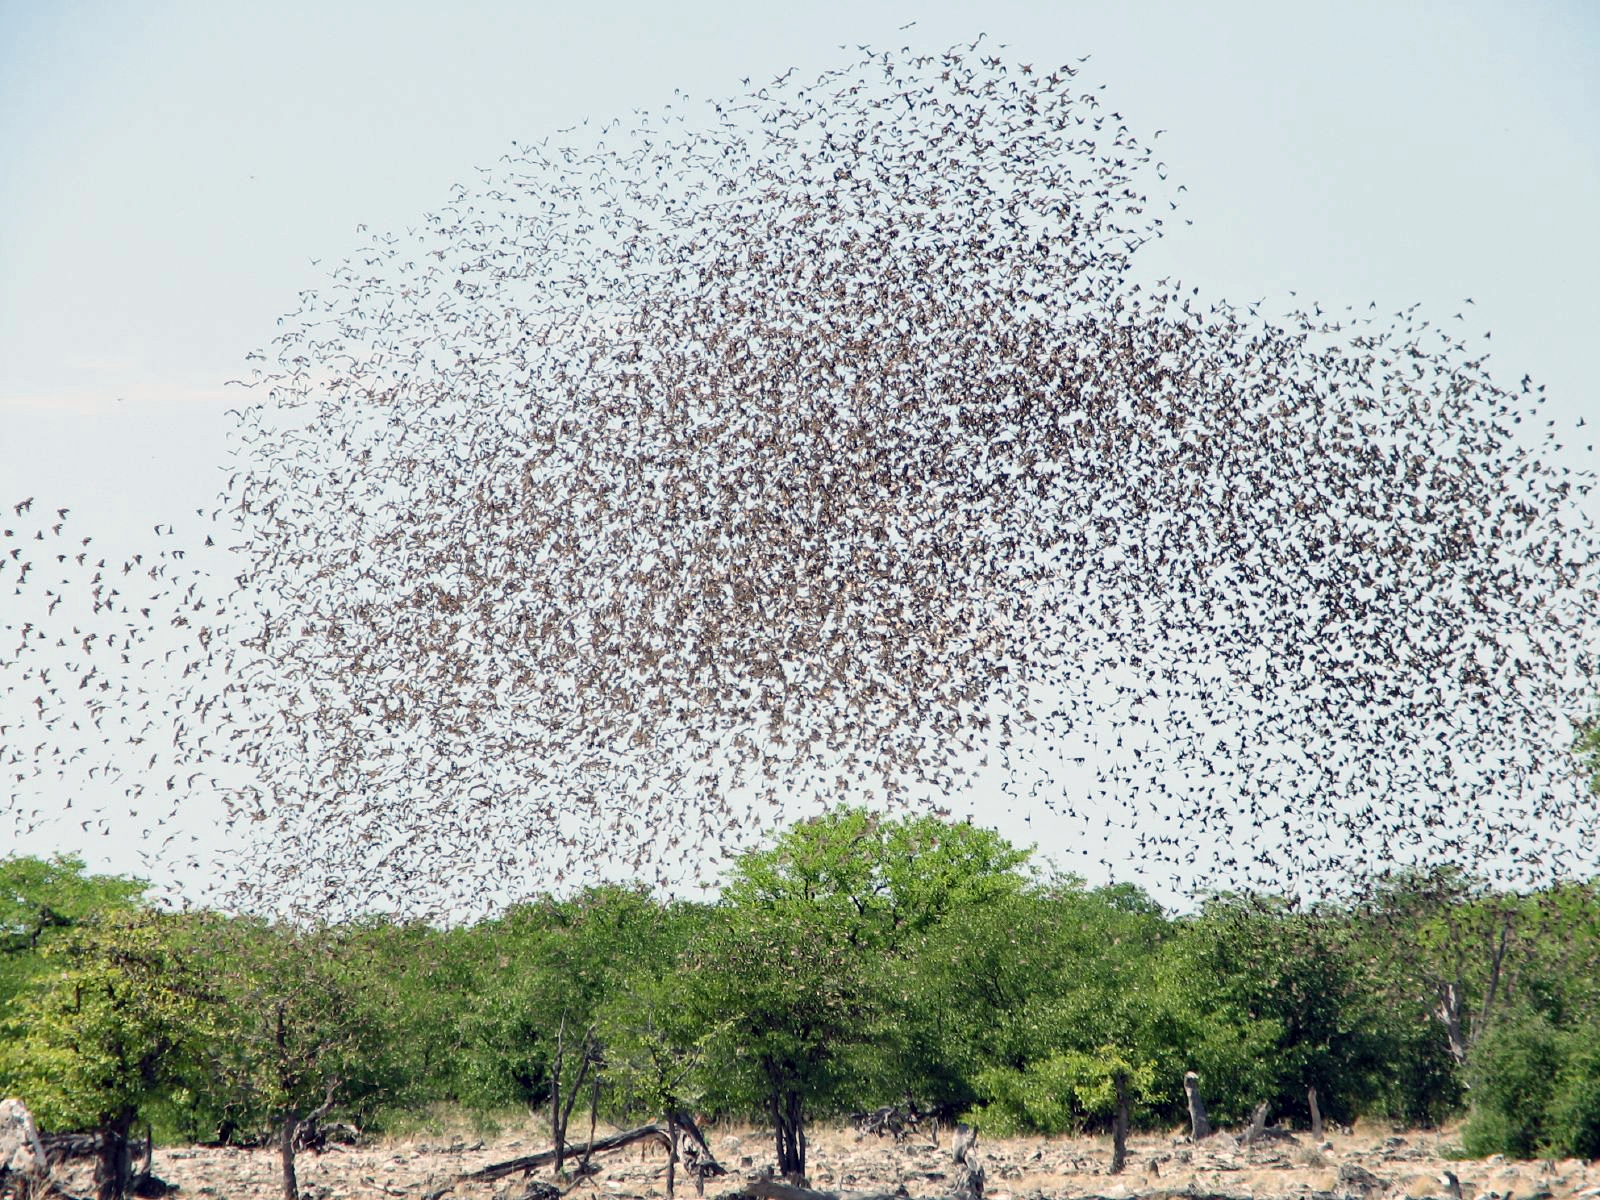
\includegraphics[width=0.4\textwidth]{resources/bandada.jpg}
    \end{figure}
\end{frame}

\begin{frame}{Fundamentos}
    El modelo se basa principalmente en dos ecuaciones:
    \begin{equation*}
        x_i(t+1) = x_i(t) + v_i(t) \Delta t
    \end{equation*}
    \begin{equation*}
        \theta(t+1) = \langle \theta(t) \rangle_r+ \Delta \theta
    \end{equation*}
    La dirección promedio se obtiene:
    \begin{equation*}
        \langle \theta(t) \rangle_r = \arctan \left( \frac{\langle \sin \theta(t) \rangle_r}{\langle \cos \theta(t) \rangle_r} \right)
\end{equation*}
\end{frame}

% Sección 2
\section{Implementación}
\begin{frame}{Arquitectura}
  Implementación:
  \begin{itemize}
      \item \textbf{Python 3}
      \item \texttt{NumPy}
      \item \texttt{Matplotlib}
  \end{itemize}
  Estructura:
  \begin{itemize}
      \item vicsek.py
      \item simulate.py
      \item simulation processing.py
      \item visualizer.py
      \item graphs.py
  \end{itemize}
\end{frame}

\begin{frame}{Diagrama de la Arquitectura}
    \begin{figure}[htbp]
        \centering
        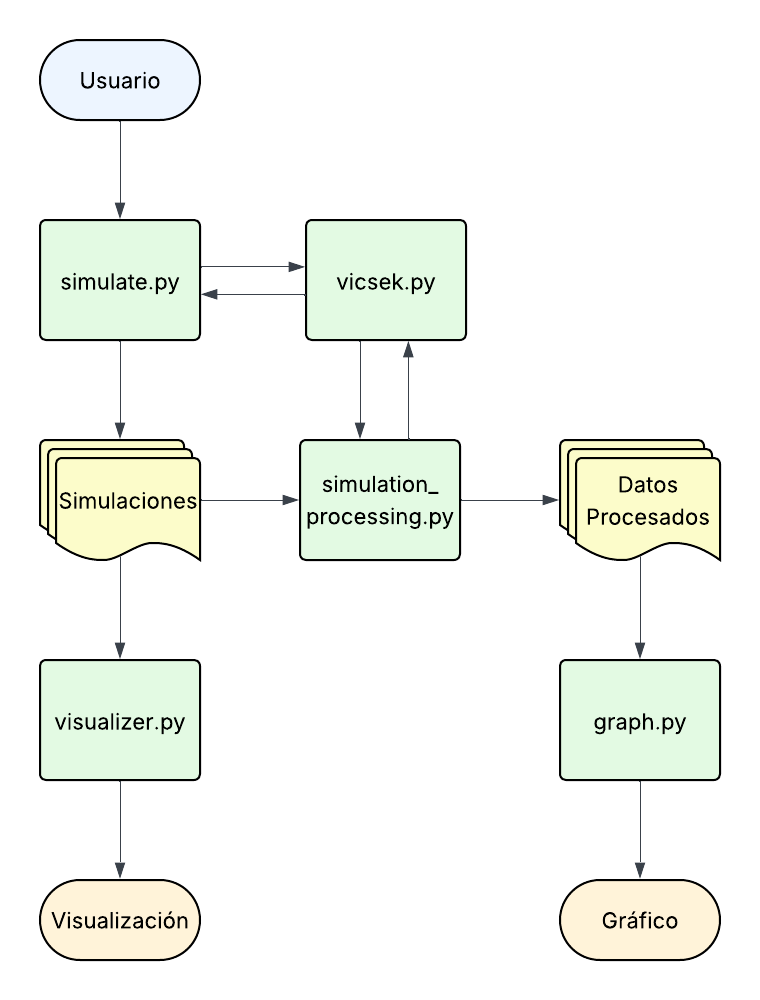
\includegraphics[width=0.45\textwidth]{resources/diagrama-uml.png}
    \end{figure}
\end{frame}

\begin{frame}{Algoritmo Implementado}
    \begin{figure}[htbp]
        \centering
        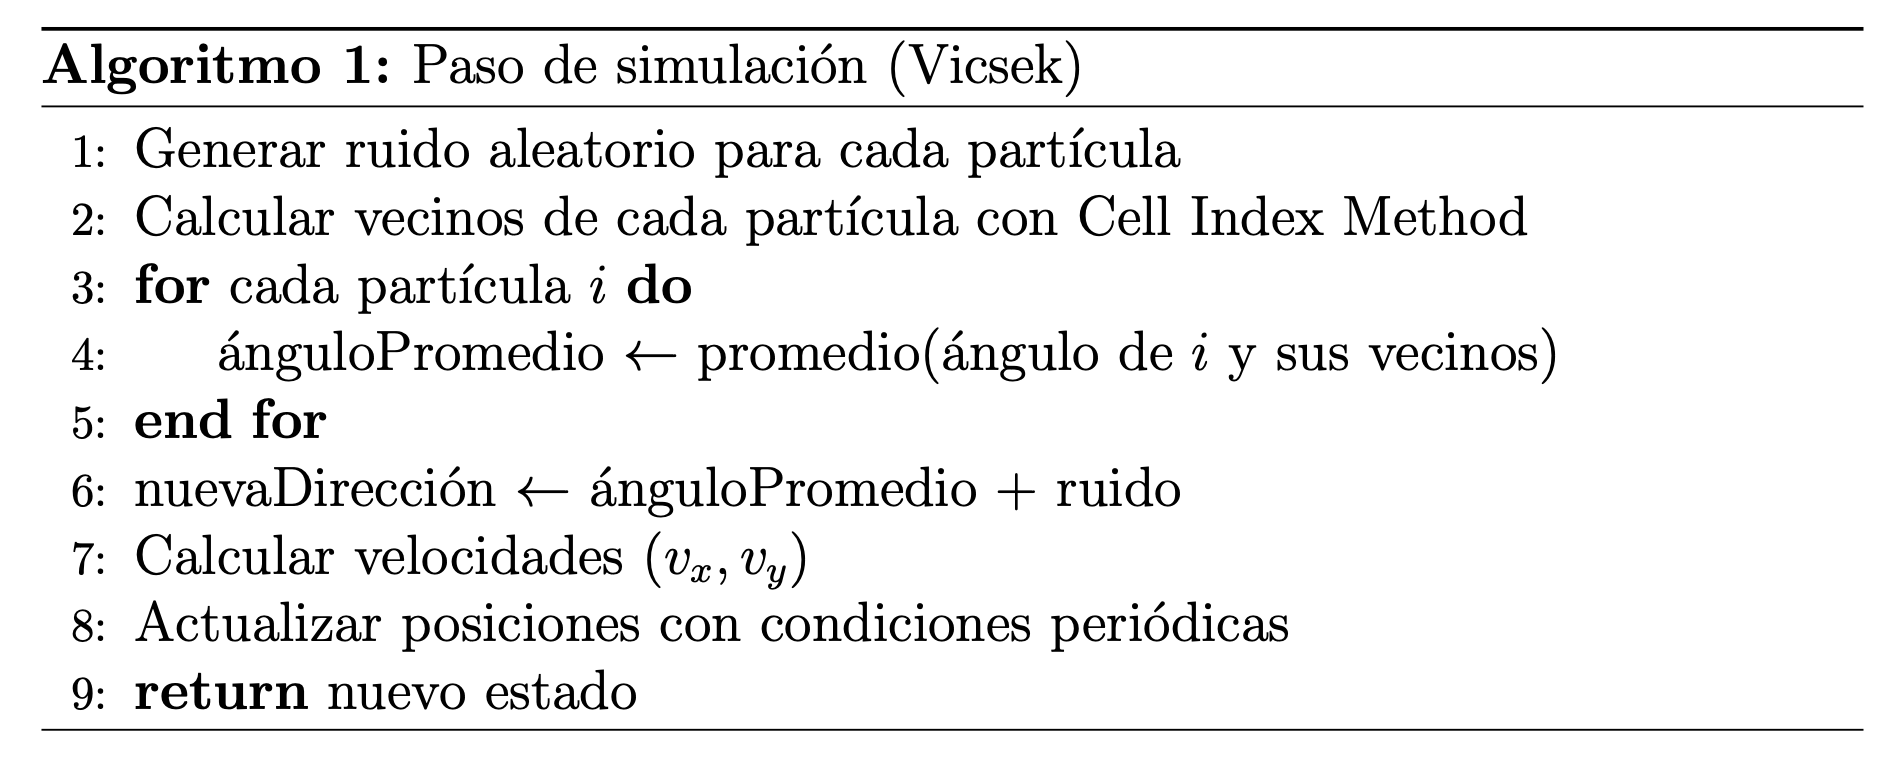
\includegraphics[width=0.9\textwidth]{resources/algorithm.png}
    \end{figure}
\end{frame}

% Sección 3
\section{Simulaciones}
\begin{frame}{Simulaciones}
    Parámetros de entrada fijos:
    \begin{itemize}
        \item $r_c=1$ - Radio de Interacción
        \item $v=0.03$ - Módulo de la Velocidad
    \end{itemize}
    Parámetros de entrada variables:
    \begin{itemize}
        \item $N\in[300,2000]$ - Cantidad de Partículas
        \item $L\in[5, 25]$ - Longitud del Lado de la Celda
        \item $T\in[300, 2000]$ - Cantidad de Pasos
        \item $\eta\in[0, 2\pi]$ - Ruido
    \end{itemize}
\end{frame}

\begin{frame}{Observable Definido}
    Parámetro de Orden $v_a(t)$
    \begin{equation*}
        v_a = \frac{1}{Nv} \left|\sum_{i=1}^{N} \vec{v_i} \right|
    \end{equation*}
    \begin{itemize}
        \item Orden: Tiende a uno.
        \item Desorden: Tiende a cero.
    \end{itemize}
    \vspace{0.5cm}
        Para cada $\eta \in \{0.1,\;0.5,\;1.0,\;2.0,\;3.14,\;4.7,\;6.28\}$ se ejecutaron 5 combinaciones de $N$ y $L$ manteniendo $\rho=4$ con $T=1000$.\\
        Luego se ejecutaron 13 simulaciones con $L=25$ y variando $N$.
\end{frame}

\begin{frame}{Desvío Estándar}
    Para las barras de error en los gráficos: Desvío Estándar
    \vspace{0.5cm}
    \begin{itemize}
        \item Sea $\{ v_a^{(1)}, v_a^{(2)}, \dots, v_a^{(M)} \}$ el conjunto de valores del observable en la región estacionaria.
        \begin{equation*}
            \overline{v_a} = \frac{1}{M} \sum_{i=1}^{M} v_a^{(i)} .
        \end{equation*}
        \item Entonces
        \begin{equation*}
            \sigma_{v_a} = \sqrt{\frac{1}{M-1} \sum_{i=1}^{M} \left( v_a^{(i)} - \overline{v_a} \right)^2 } .
        \end{equation*}
    \end{itemize}
\end{frame}

\begin{frame}{Interacción Tipo Votante}
    Ahora, cada partícula copia la dirección de un único vecino elegido al azar dentro de su radio de interacción.\\
    \vspace{0.5cm}
    Simulaciones:
    \begin{itemize}
        \item 5 simulaciones con $T=2000$ para $N=300$ y $L=10$ variando $\eta$ en $[0;0.5]$.
        \item 11 simulaciones con $T=$ para $L=10$ y $\eta=0$ variando $N$ en $[300;2000]$.
    \end{itemize}
\end{frame}

% Sección 4
\section{Resultados}
\begin{frame}{Animaciones del Sistema}
    \begin{minipage}[t]{0.60\textwidth}
        \begin{figure}[H!]
            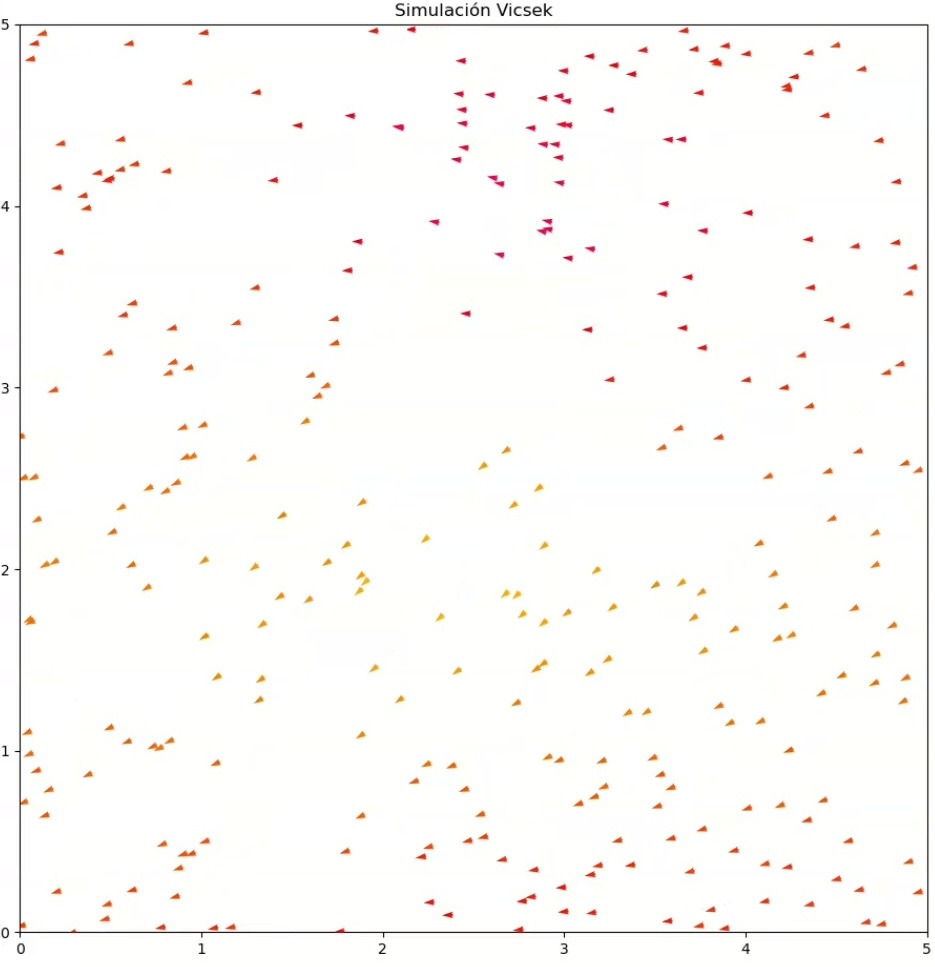
\includegraphics[height=.65\textheight]{resources/animacion-eta-0.1.jpeg}
            \caption*{\href{https://youtube.com/shorts/tTuYZXHlj-A}{Link a la animación completa.}}
            \label{animacion-eta-0.1}
        \end{figure}
    \end{minipage}
    \hfill
    \begin{minipage}[t]{0.30\textwidth}
        \begin{block}{Datos del Sistema}
            \begin{itemize}
                \item $N=300$
                \item $L=5$
                \item $T=300$
                \item $\eta=0.1$
            \end{itemize}
        \end{block}
    \end{minipage}
\end{frame}

\begin{frame}{Animaciones del Sistema}
    \begin{minipage}[t]{0.60\textwidth}
        \begin{figure}[H!]
            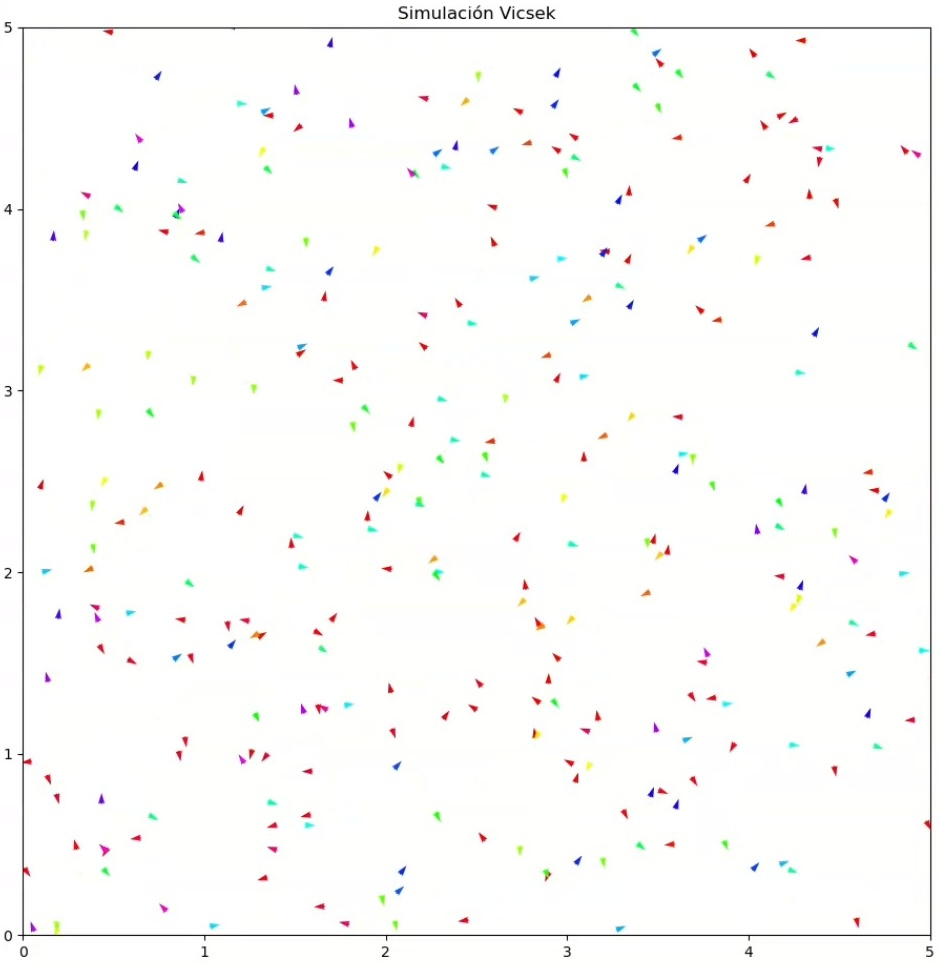
\includegraphics[height=.65\textheight]{resources/animacion-eta-2pi.jpeg}
            \caption*{\href{https://youtube.com/shorts/hZ2bDILFapQ}{Link a la animación completa.}}
            \label{animacion-eta-2pi}
        \end{figure}
    \end{minipage}
    \hfill
    \begin{minipage}[t]{0.35\textwidth}
        \begin{block}{Datos del Sistema}
            \begin{itemize}
                \item $N=300$
                \item $L=5$
                \item $T=300$
                \item $\eta=6.28 (\approx2\pi)$
            \end{itemize}
        \end{block}
    \end{minipage}
\end{frame}

\begin{frame}{Animaciones del Sistema}
    \begin{minipage}[t]{0.60\textwidth}
        \begin{figure}[H!]
            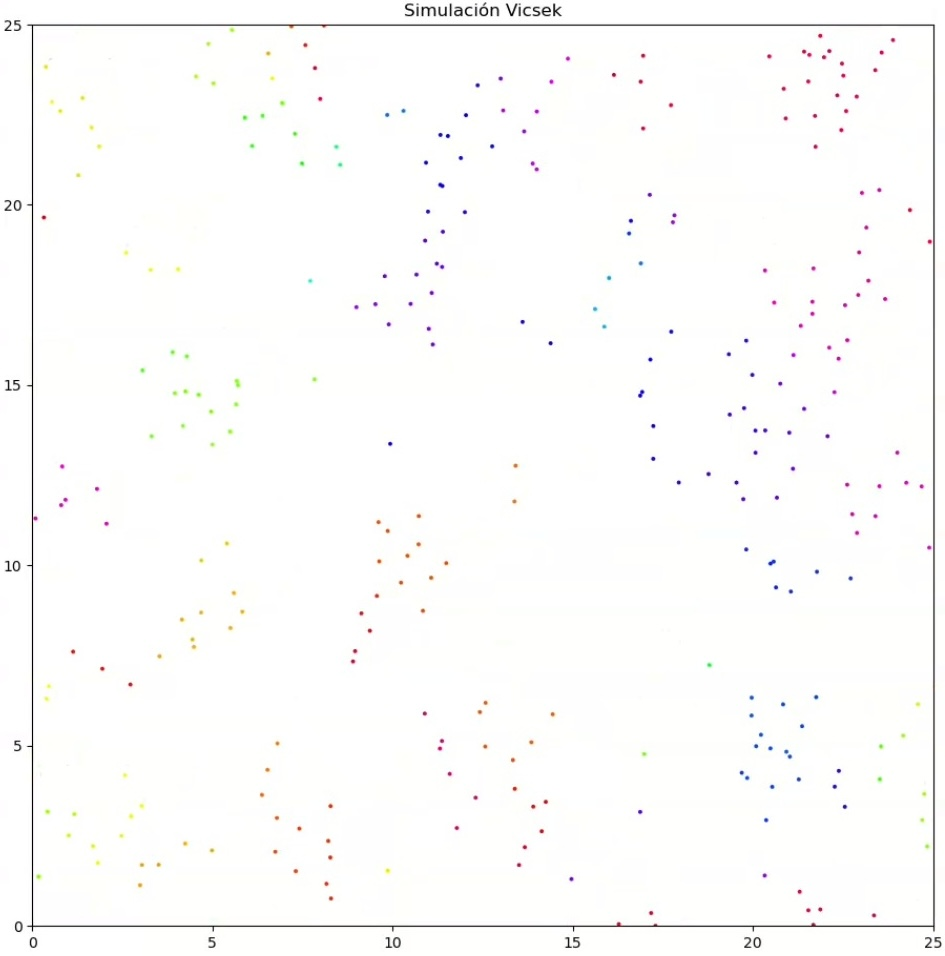
\includegraphics[height=.65\textheight]{resources/animacion-l-25.jpeg}
            \caption*{\href{https://www.youtube.com/shorts/jTQ0DtBW6Tg}{Link a la animación completa.}}
            \label{animacion-l-25}
        \end{figure}
    \end{minipage}
    \hfill
    \begin{minipage}[t]{0.35\textwidth}
        \begin{block}{Datos del Sistema}
            \begin{itemize}
                \item $N=300$
                \item $L=25$
                \item $T=300$
                \item $\eta=0.1$
            \end{itemize}
        \end{block}
    \end{minipage}
\end{frame}

\begin{frame}{Evolución Temporal del Observable}
    \begin{figure}[H!]
        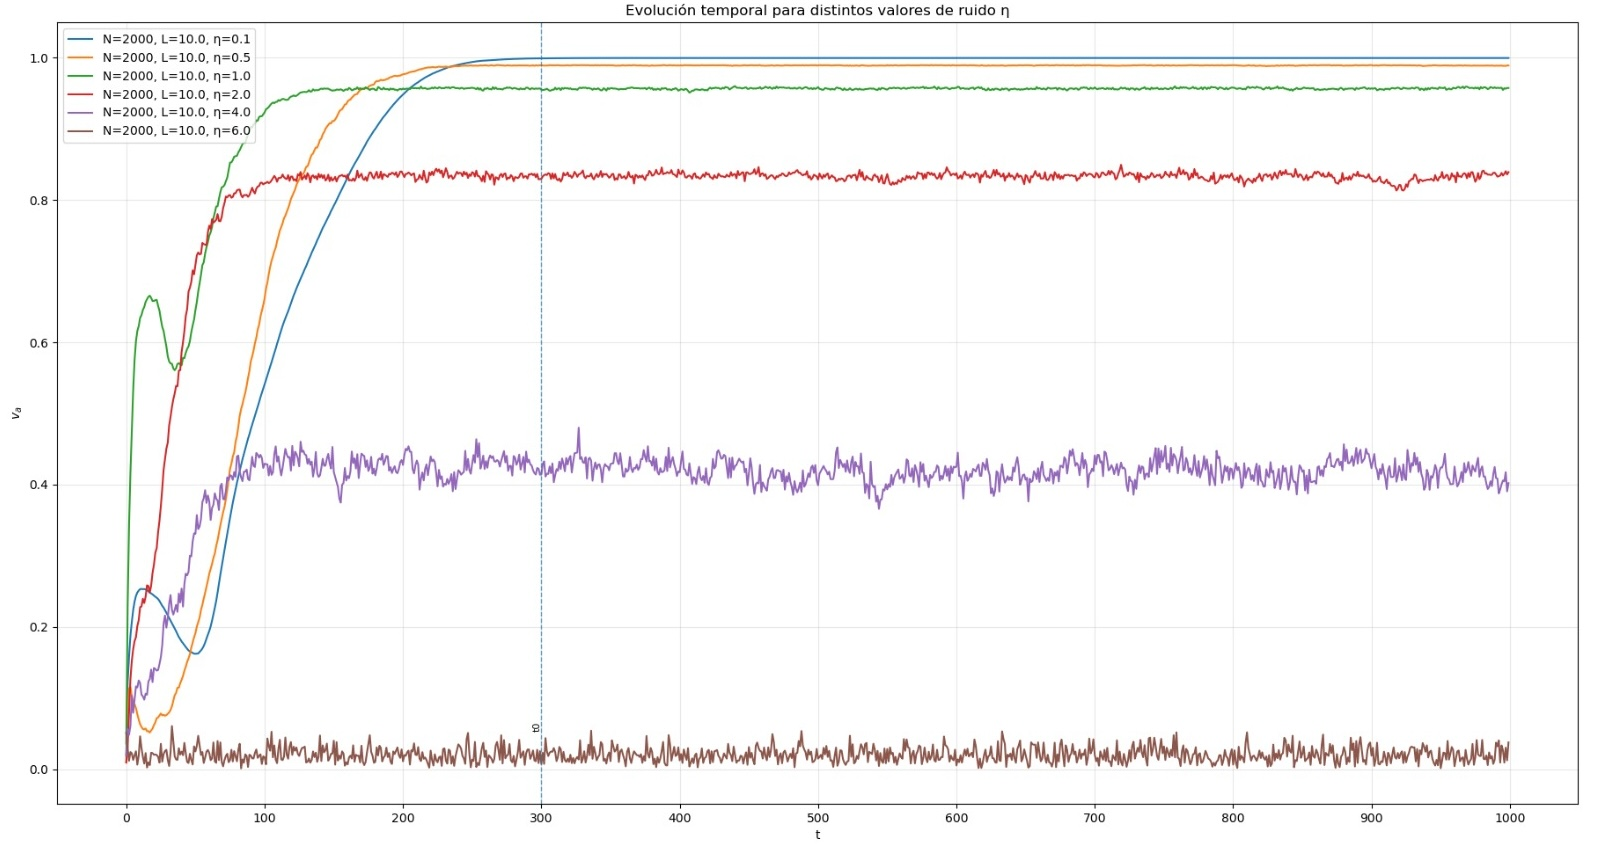
\includegraphics[height=.65\textheight]{resources/grafico-va-t.jpeg}
        \label{grafico-va-t}
    \end{figure}
\end{frame}

\begin{frame}{Relación entre el Ruido del Sistema y el Observable}
    \begin{figure}[H!]
        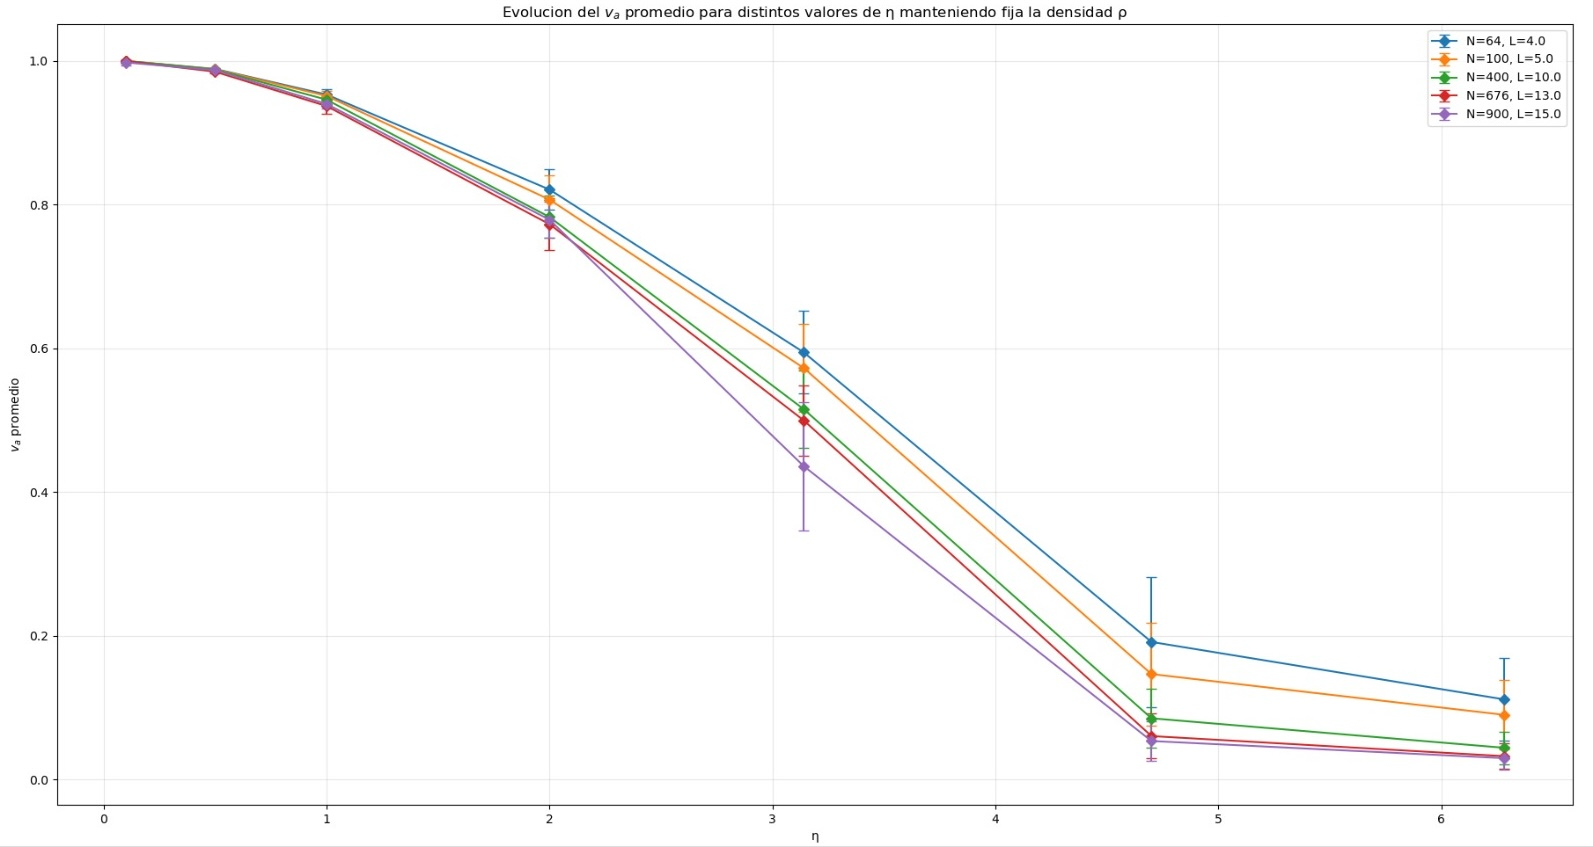
\includegraphics[height=.65\textheight]{resources/grafico-va-eta.jpeg}
        \label{grafico-va-eta}
    \end{figure}
    \begin{beamercolorbox}[sep=5pt,center]{block body}
        \begin{minipage}[t]{0.45\textwidth}
            \centering
            \small{$\rho=4$}
        \end{minipage}
        \hfill
        \begin{minipage}[t]{0.45\textwidth}
            \centering
            \small{$T=1000$}
        \end{minipage}
    \end{beamercolorbox}
\end{frame}

\begin{frame}{Relación entre el Ruido del Sistema y el Observable}
    \begin{figure}[H!]
        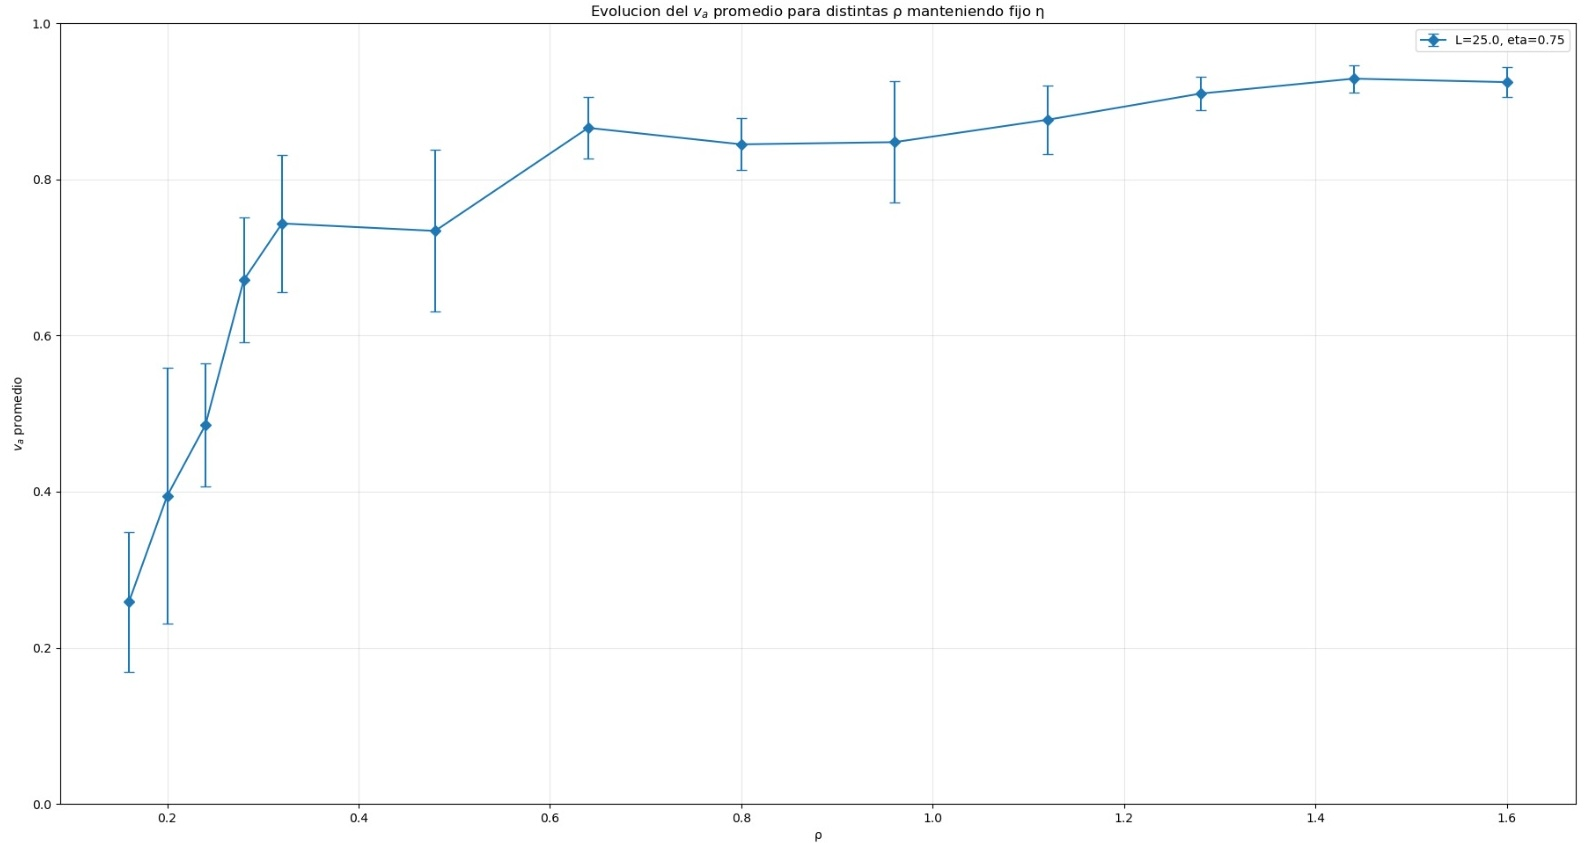
\includegraphics[height=.65\textheight]{resources/grafico-va-rho.jpeg}
        \label{grafico-va-rho}
    \end{figure}
    \centering
    \begin{beamercolorbox}[sep=5pt,center]{block body}
        \scriptsize
        $N \in \{100,\,125,\,150,\,175,\,200,\,300,\,400,\,500,\,600,\,700,\,800,\,900,\,1000\}$
    \end{beamercolorbox}
\end{frame}

\begin{frame}{Interacción Tipo Votante}
    \begin{minipage}[t]{0.60\textwidth}
        \begin{figure}[H!]
            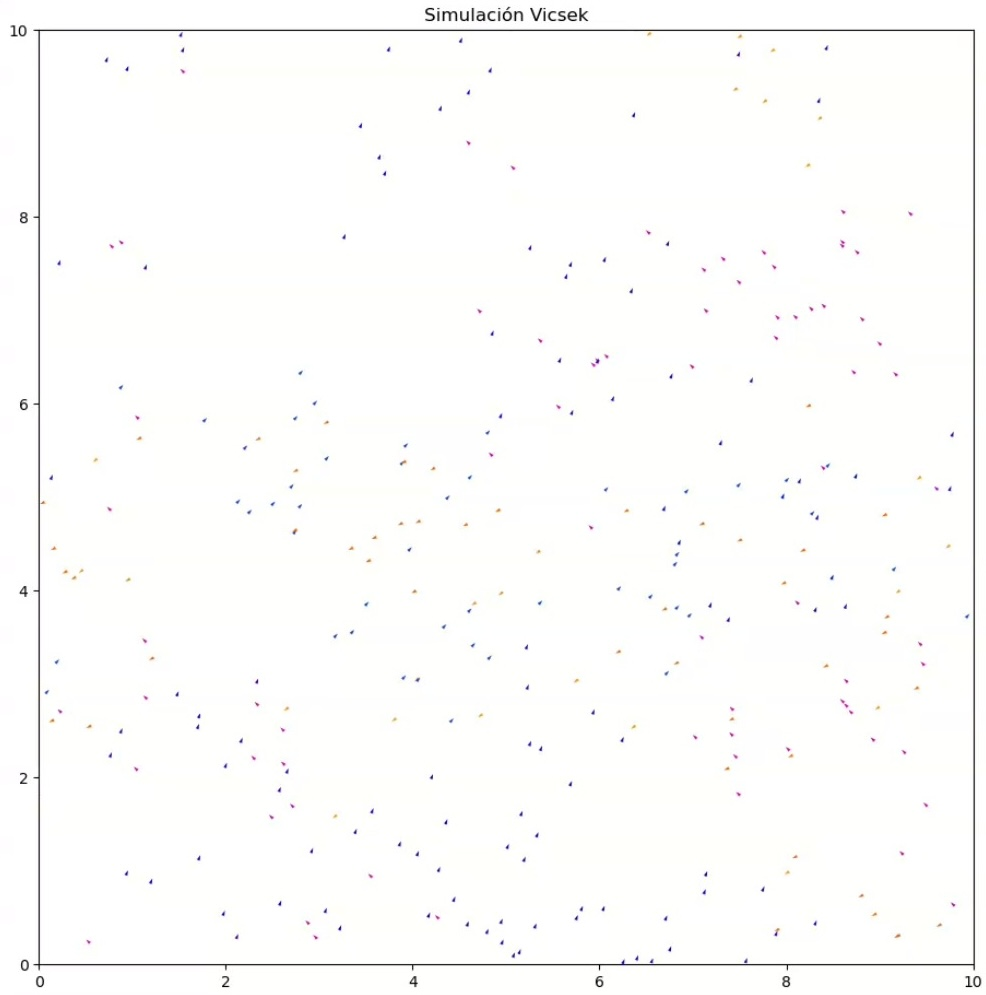
\includegraphics[height=.65\textheight]{resources/animacion-votante-n-300.jpeg}
            \caption*{\href{https://www.youtube.com/shorts/W_7f7Aq2uGs}{Link a la animación completa.}}
            \label{animacion-votante-n-300}
        \end{figure}
    \end{minipage}
    \hfill
    \begin{minipage}[t]{0.35\textwidth}
        \begin{block}{Datos del Sistema}
            \begin{itemize}
                \item $N=300$
                \item $L=10$
                \item $T=2000$
                \item $\eta=0$
            \end{itemize}
        \end{block}
    \end{minipage}
\end{frame}

\begin{frame}{Interacción Tipo Votante}
    \begin{minipage}[t]{0.60\textwidth}
        \begin{figure}[H!]
            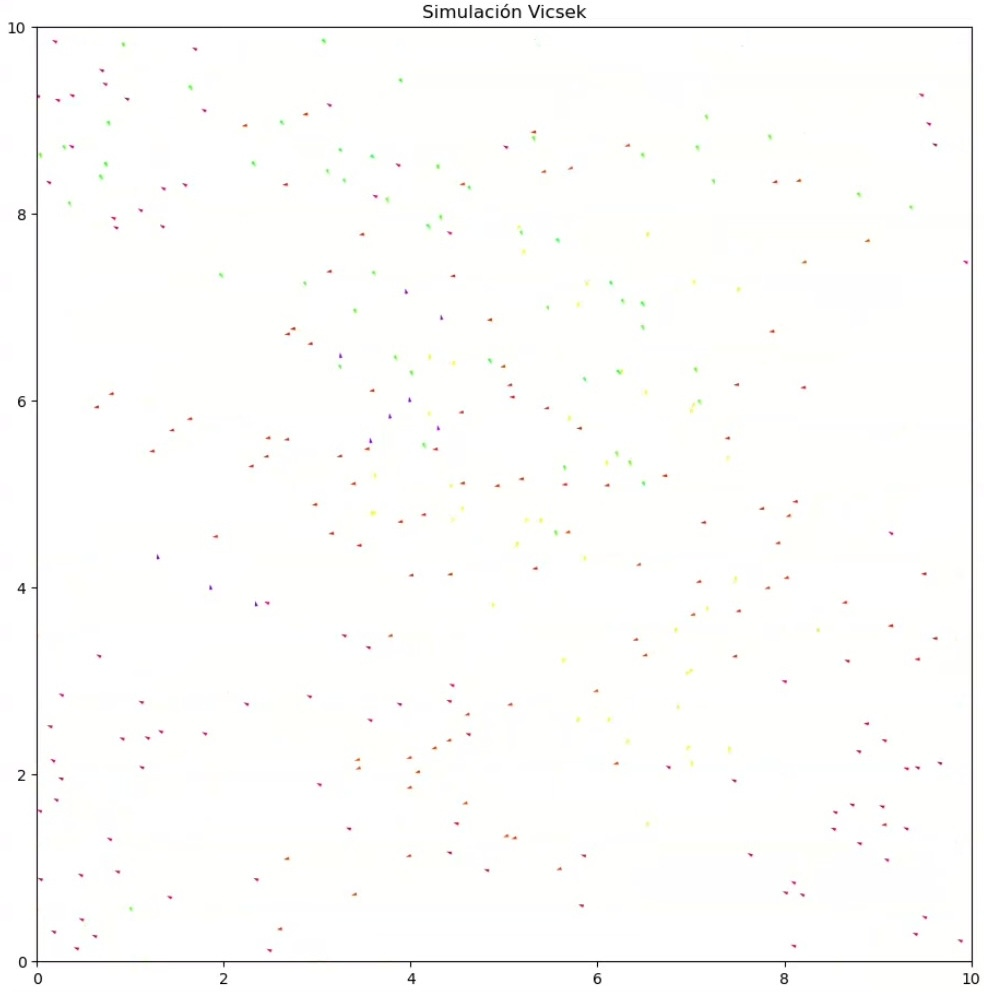
\includegraphics[height=.65\textheight]{resources/animacion-votante-n-300-eta.jpeg}
            \caption*{\href{https://www.youtube.com/shorts/x6ymonK0mbM}{Link a la animación completa.}}
            \label{animacion-votante-n-300-eta}
        \end{figure}
    \end{minipage}
    \hfill
    \begin{minipage}[t]{0.35\textwidth}
        \begin{block}{Datos del Sistema}
            \begin{itemize}
                \item $N=300$
                \item $L=10$
                \item $T=2000$
                \item $\eta=0.05$
            \end{itemize}
        \end{block}
    \end{minipage}
\end{frame}

\begin{frame}{Interacción Tipo Votante}
    \begin{figure}[H!]
        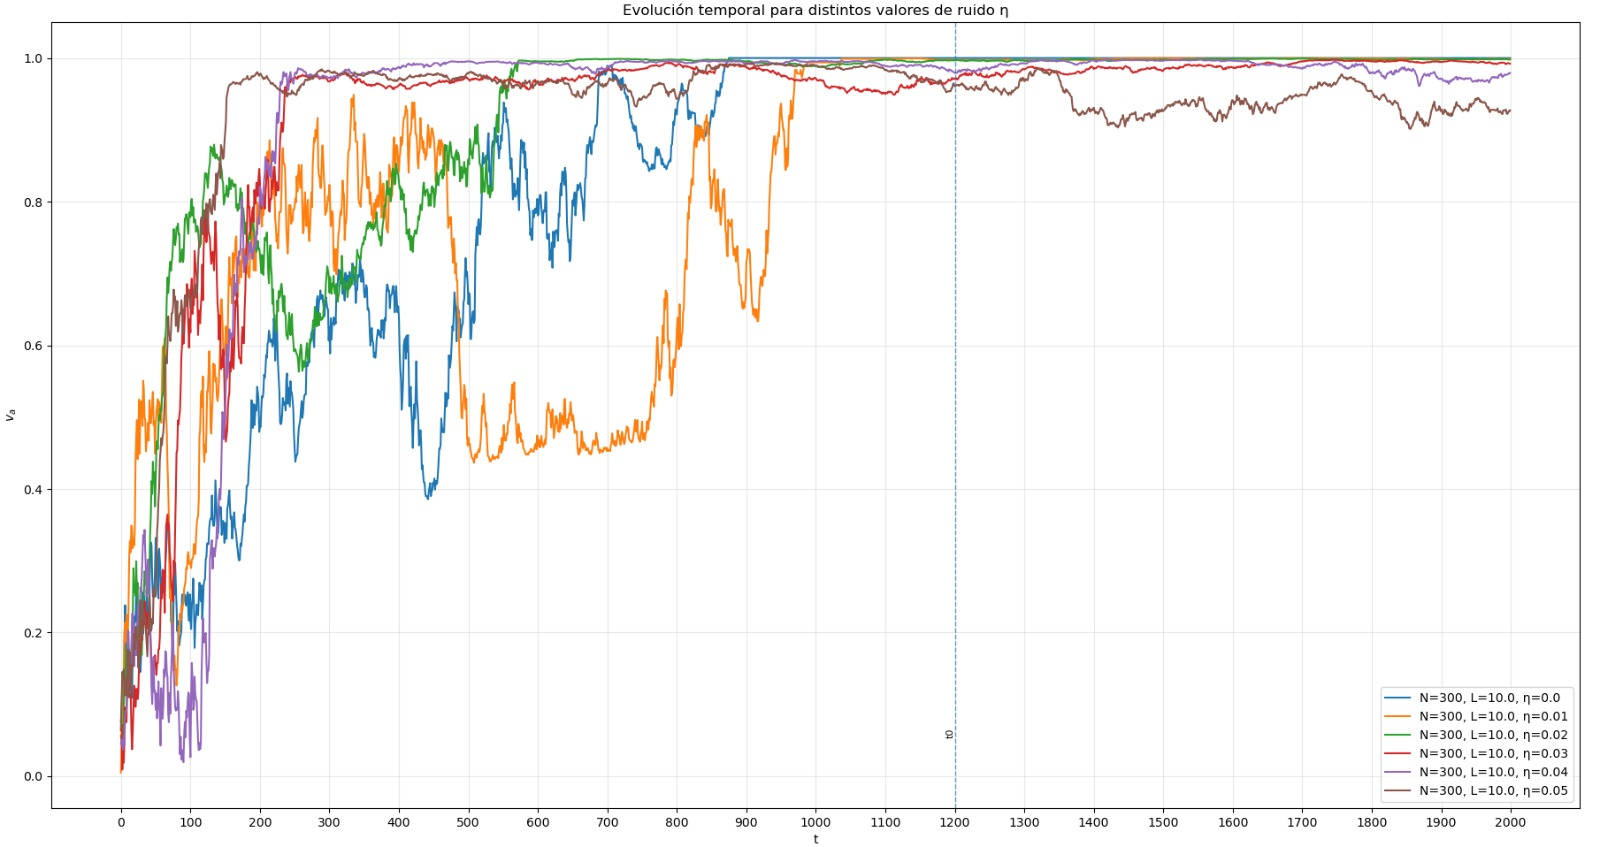
\includegraphics[height=.65\textheight]{resources/grafico-votante-va.jpeg}
        \label{grafico-votante-va}
    \end{figure}
\end{frame}

\begin{frame}{Interacción Tipo Votante}
    \begin{figure}[H!]
        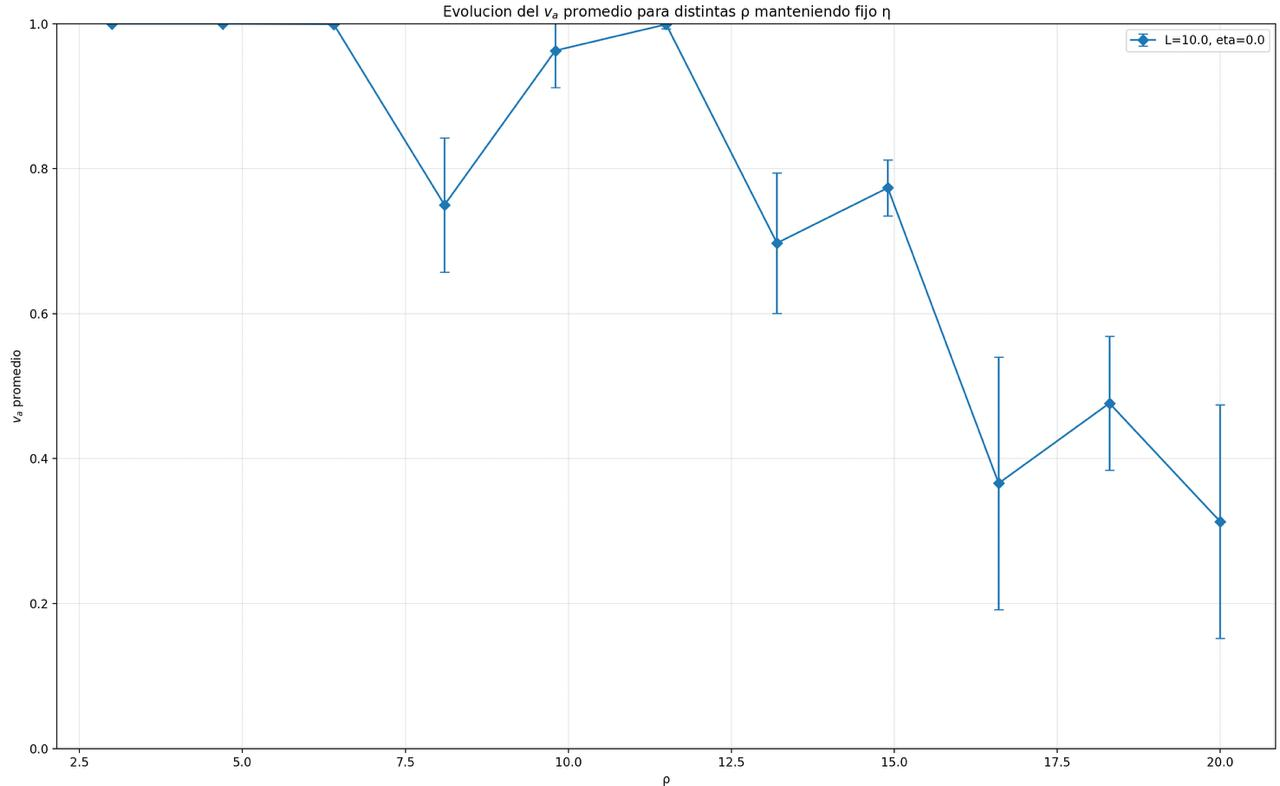
\includegraphics[height=.65\textheight]{resources/grafico-votante.jpeg}
        \label{grafico-votante}
    \end{figure}
    \begin{beamercolorbox}[sep=5pt,center]{block body}
        \scriptsize
        $N \in \{300,\,470,\,640,\,810,\,980,\,1150,\,1320,\,1490,\,1660,\,1830,\,2000\}$
    \end{beamercolorbox}
\end{frame}

% Sección 5
\section{Conclusiones}
\begin{frame}{Conclusiones}
    Algunas conclusiones obtenidas:
    \begin{itemize}
        \item El parámetro de orden $v_a$ depende en gran medida del nivel de ruido $\eta$.
        \item Al aumentar $N$ manteniendo fijo $L$, se favorece la formación de un mayor orden colectivo.
        \item Contraste con la regla de interacción tipo votante.
    \end{itemize}
\end{frame}

\begin{frame}
    \begin{beamercolorbox}[sep=8pt,center]{title}
        \usebeamerfont{title} Muchas gracias
    \end{beamercolorbox}
\end{frame}
\end{document}
